\documentclass[10pt,a4paper,twocolumn,twoside]{article}
\usepackage[utf8]{inputenc}
\usepackage[catalan]{babel}
\usepackage{multicol}
\usepackage{graphicx}
\usepackage{fancyhdr}
\usepackage{times}
\usepackage{titlesec}
\usepackage{url}
\usepackage{multirow}
\usepackage{lettrine}
\usepackage[top=2cm, bottom=1.5cm, left=2cm, right=2cm]{geometry}
\usepackage[figurename=Fig.,tablename=TAULA]{caption}
\usepackage{mathtools}
\captionsetup[table]{textfont=sc}

\author{\LARGE\sffamily Miquel Freixes Faya}
\title{\Huge{\sffamily Anàlisis de la relació entre les emisions de gasos hivernacle i l'augment de la temperatura, mitjançant algoritmes i tecnologies de Big Data}}
\date{}

\newcommand\blfootnote[1]{%
  \begingroup
  \renewcommand\thefootnote{}\footnote{#1}%
  \addtocounter{footnote}{-1}%
  \endgroup
}

%
%\large\bfseries\sffamily
\titleformat{\section}
{\large\sffamily\scshape\bfseries}
{\textbf{\thesection}}{1em}{}

\begin{document}

\fancyhead[LO]{\scriptsize MIQUEL FREIXES FAYA: ANÀLISIS DE LA RELACIÓ ENTRE LES EMISIONS DE GASOS HIVERNACLE I L'AUGMENT DE LA TEMPERATURA}
\fancyhead[RO]{\thepage}
\fancyhead[LE]{\thepage}
\fancyhead[RE]{\scriptsize EE/UAB TFG INFORMÀTICA: ANÀLISIS DE LA RELACIÓ ENTRE LES EMISIONS DE GASOS HIVERNACLE I L'AUGMENT DE LA TEMPERATURA}

\fancyfoot[CO,CE]{}

\fancypagestyle{primerapagina}
{
   \fancyhf{}
   \fancyhead[L]{\scriptsize TFG EN ENGINYERIA INFORMÀTICA, ESCOLA D'ENGINYERIA (EE), UNIVERSITAT AUTÒNOMA DE BARCELONA (UAB)}
   \fancyfoot[C]{\scriptsize ``Febrer'' de 2019, Escola d'Enginyeria (UAB)}
}

%\lhead{\thepage}
%\chead{}
%\rhead{\tiny EE/UAB TFG INFORMÀTICA: TÍTOL (ABREUJAT SI ÉS MOLT LLARG)}
%\lhead{ EE/UAB \thepage}
%\lfoot{}
%\cfoot{\tiny{February 2015, Escola d'Enginyeria (UAB)}}
%\rfoot{}
\renewcommand{\headrulewidth}{0pt}
\renewcommand{\footrulewidth}{0pt}
\pagestyle{fancy}

%\thispagestyle{myheadings}
\twocolumn[\begin{@twocolumnfalse}

%\vspace*{-1cm}{\scriptsize TFG EN ENGINYERIA INFORMÀTICA, ESCOLA D'ENGINYERIA (EE), UNIVERSITAT AUTÒNOMA DE BARCELONA (UAB)}

\maketitle

\thispagestyle{primerapagina}
%\twocolumn[\begin{@twocolumnfalse}
%\maketitle
%\begin{abstract}
\begin{center}
\parbox{0.915\textwidth}
{\sffamily
\textbf{Resum--}
L'emisió de gasos hivernacle per part de la humanitat ha estat afectant negativament les temperatures del planeta i augmentant l'efecte del canvi climatic. L'impacte es tant elevat que cada cop hi ha temperatures més elevades, més desertificacions, augment del nivell del mar... Al llarg del temps s'han fet múltiples estudis demostrant i explicant que el canvi climàtic es un fet i que cal actuar d'immediat, pero encara hi ha molta gent reticent a admetre que existeix aquest canvi climàtic o que té relació amb l'humanitat. Aquest treball es un altre intent de demostrar que aquest fet existeix i ho fa aplicant tècniques de \textit{Machine Learning} i \textit{Big Data} per tal de relacionar aquest augment de la temperatura amb una de les seves causes principals, l'emisisó de gasos hivernacle per part de l'èsser humà.
\\
\\
\textbf{Paraules clau-- } Aprenentatge Computacional, Conjunt de dades, Hiperparàmetres, Regressió màxim 2 línies \\
\\
%\end{abstract}
%\bigskip
%\begin{abstract}
\bigskip
\\
\textbf{Abstract--} The release of greenhouse gases by the humanity it is influencing in a negative way the temperatures of the planet and increasing the effect of the climate change. The magnitude of this impact is such that the temperatures are constantly increasing, there is more desertification, the level of the sea is increasing... Over time there has been multiple studies proving and explaining that climate change is a fact and that we have to act against as soon as possible. But there are people that still don't believe in the existence of it or how this can be relate it with humanity. This project is another chance to demonstrate that climate change exists, to do it applies teh techniques of Machine Learning and Big Data in order to link the incrase of the temperatures with one of the main causes, the release of greenhouse gases by the human being.
\\
\\
\textbf{Keywords-- } Machine Learning, DataSet, Hyperparameters, Regresion\\
}

\bigskip

{\vrule depth 0pt height 0.5pt width 4cm\hspace{7.5pt}%
\raisebox{-3.5pt}{\fontfamily{pzd}\fontencoding{U}\fontseries{m}\fontshape{n}\fontsize{11}{12}\selectfont\char70}%
\hspace{7.5pt}\vrule depth 0pt height 0.5pt width 4cm\relax}

\end{center}

\bigskip
%\end{abstract}
\end{@twocolumnfalse}]

\blfootnote{$\bullet$ E-mail de contacte: m.freixes.faya@gmail.com}
\blfootnote{$\bullet$ Menció realitzada: Tecnologies de la Informació}
\blfootnote{$\bullet$ Treball tutoritzat per: Jordi Casas Roma (DEIC)}
\blfootnote{$\bullet$ Curs 2018/19}
\section{Introducció}
\lettrine[lines=3]{E}{n} els últims anys la temperatura de la Terra no ha parat d'augmentar en la gran majoria de la seva superfície, efecte resultant del canvi climàtic. Alguns estudis demostren que des del 1980 hi ha hagut un increment d'1ºC en la temperatura de tota la Terra [1]. Encara que 1ºC no sembli significant s'ha de contextualitzar, cal incidir en el fet de que s'està parlant sobre tota la superficie terrestre, inclosos oceans, per tant que augmenti 1ºC significa que el canvi de temperatura s'ha vist reflectit en l'aigua, els pols, els deserts... Les consequencies d'això ja s'estant fent evidents en molts indrets, hi ha desertificació en molts països, els pols s'estan desfent a un ritme alarmant... 

S'ha demostrat innomerables cops que aquests fets tenen diferents causes que els originen i que una de les més preocupants es la contaminació produida pels essers humans. Dins d'aquesta contaminació tenen un paper molt important les emisions dels gasos hivernacle. Aquests gasos sempre han estat presents en l'atmosfera, pero des de la revolució industrial la seva presencia en l'atmosfera s'ha vist incrementada enormement. Això provoca que les radiacions solars travessin l'atmosfera i que la superficie les absorbeixi. Actualment hi ha molts estudis sobre aquestes emisions i hi ha moltes dades de sensors que han anat registrant les emisions de cada país al llarg dels anys. Al mateix temps, hi ha molts conjunts de dades sobre les temperatures mitjanes mensuals de cada país des de fa anys. Es podria trobar alguna relació entre les emisions de gasos hivernacle i les temperatures per poder predir les temperatures dels proxims anys? A partir de les emisions i diverses temperatures anteriors, un algorisme pot predir les temperatures dels proxims mesos?

Aquest document està dividit en diverses seccions. A la secció 2 s'expliquen els objectius del treball. A la 3a secció s'explica l'estat de l'art sobre les tècniques de Machine Learning i en la 4a la metodologia que s'ha seguit al llarg del treball. Per acabar a la 5a secció està explicat el desenvolupament, seguidament de l'anàlisis de resultats a la secció 6. Per acabar a la secció 7 es troben les conclusions i a la 8a secció hi ha les propostes per futurs treballs.   
\section{Objectius}
L'objectiu principal d'aquest treball és analitzar el comportament de diferents algorismes, de Machine Learning (ML), a l'hora de predir la temperatura d'un país a partir de les seves emissions de gassos hivernacle. Aquest objectiu es limitarà als països del continent d'Europa i al periode composat entre els anys del 1990 al 2013. L'objectiu principal es pot desglosar en diferents subobjectius que s'han d'aconseguir per arribar a satisfer-lo:
\begin{itemize}
\item Crear un DataSet que relacioni els països amb les seves temperatures i les seves emisions a partir de dades extretes de fonts fiables i lliures de drets. Aquest ha de tenir les suficients dades per poder entrenar els algorismes de ML apropiadament .
\item Analitzar quins son els algorismes de ML més utilitzats actualment en problemes de regressió i implementar-los correctament.
\item Trobar la millor configuració de cada un d'ells aplicant mètodes utilitzats en Big Data, com el GridSearch o el RandomizedSearch.
\item Poder determinar el millor algorisme dels diversos seleccionats i poder extreure els diferents resultats de forma gràfica i entenedora.     
\end{itemize}
\section {Estat de l'art}
En aquests darrers anys el Big Data ha passat a ser un dels termes més utilitzats en molts àmbits més enllà de la informàtica, com per exemple, la medicina o l'economia.  
EXPLICAR XARXES, FER ESQUEMA DE NEURONES INTERCONNECTADES, EXPLICAR TECNOLOGIES COM TENSORFLOW I SCIKIT, SPARK I PANDAS... TOT MOLT PER SOBRE I ALA
\section {Metodologia}
A l'hora de fer projectes hi ha un gran nombre de metodologies per escollir, però en l'àmbit de la informàtica les més utilitzades són les Agile. Això és degut a l'increment del nombre de projectes àgils acabats en èxit, respecte dels projectes on s'han aplicat les metodologies tradicionals. [2] Dins de la metodologia àgil hi ha diverses metodologies com Scrum, Kanban, XP... En aquest treball se seguirà la Kanban, a causa del fet que la metodologia Scrum no es podria aprofitar al màxim amb només una persona en el projecte. La principal raó per no escollir Scrum ha estat que molts papers els hauria de fer la mateixa persona, com el de Scrum Master, Product Owner... Algunes de les principals característiques no tindrien sentit. [3]

Kanban es basa en una taula de progrés on es fiquen les tasques per fer, les que s'estan fent i les fetes. Això permetrà un seguiment constant de com avança el projecte. També permet treballar segons prioritats, no per temps, i això s'ajusta molt bé al tipus de projecte que es desenvoluparà. Degut al fet que el projecte està format per tasques que es poden paral·lelitzar, i d'altres que no es poden fer sense una prèvia, apareixeran prioritats al llarg del desenvolupament. [4]

La fase del projecte destinada a l'anàlisi dels datasets es farà utilitzant el software d'Apache Spark a partir de Databricks. S'ha escollit Databricks perquè ofereix un petit clúster amb 6Gb de Ram gratuïtament per estudiants, uns recursos més que suficients per processar el volum de dades desitjat.
A part d'això, tot el progrés de cada etapa s'anirà guardant en un Git per tal de no perdre res i poder mantenir un històric dels canvis. En el Git es guardarà els informes, els codis i algorismes necessaris i els datasets amb les dades.
Per acabar, els codis es faran en el llenguatge de Python. Aquest llenguatge és molt utilitzat a l'hora de treballar amb algorismes de Machine Learning. A més, s'utilitzaran algorismes de la pàgina web de Scikit Learn, a causa de la gran varietat d'algorismes que ofereix i a la facilitat d'implementar-los. No obstant això, el desenvolupament de les xarxes neuronals es farà en Keras. Això es degut a que Keras permet treballar amb més detall l'implementació de les xarxes i es una API que treballa sobre TensorFlow, per tant es troba en l'estat de l'art de l'àmbit del \textit{Deep Learning}.
\section {Desenvolupament}
\subsection{Preprocessament de dades}
Per començar s'han importat els dos \textit{DataSets} des del seu csv corresponent:
El primer està format de quatre columnes, tal com es mostra a la taula 1 hi ha una amb la data, en format String amb dies mesos i anys. El segon valor és la temperatura mesurada amb un marge d'error del 95\%, serà el valor que es donarà per vàlid al llarg del treball. El tercer és el marge d'error que pot tenir la temperatura de la segona columna i l'última el nom del país al qual s'està mesurant les temperatures. Aquest \textit{DataSet} està extret de Kaggle, però és una recopilació d'investigacions fetes per Berkeley Earth [5]. És una empresa sense ànim de lucre destinada a revisar i documentar l'increment de temperatura al llarg dels anys. Aquest \textit{DataSet} és una compressió de dades extretes de més d'1,6 bilions de registres entre els anys 1750 i el 2013 de tot el món per cada mes de l'any.
\begin{table}[ht]
\caption{Taula de temperatures}
\begin{center}
\begin{tabular}{c c c c} % centered columns (4 columns)
\hline\hline %inserts double horizontal lines
dt & Temp & Average & Country \\
\hline
01-01-1750 & 1.12 & 2.245 & Germany \\
01-02-1750 & 2.234 & 1.3 & Germany \\
\hline
\end{tabular}
\end{center}
\end{table}

El segon està compost pel mateix nombre de columnes. Com es pot veure a la taula 2, és bastant semblant a l'anterior. La primera és el nom del país on s'està mesurant, la segona és l'any on s'ha mesurat, aquest cop en format d'enter. En la tercera tenim el valor de la mitjana de Kilotones de gas produït per capita en el país, i en l'última tenim el tipus de gas que s'ha mesurat i quins paràmetres s'han utilitzat per fer-ho. En aquest \textit{DataSet} s'han extret les dades de les emissions de cada país, dels diferents gasos hivernacle des de l'any 1990 al 2013 [6]. La majoria de mesures estan extretes sense considerar les activitats d'ús de la terra o d'intercanvi de recursos amb la terra, anomenades en anglès com a LULUCF (\textit{Land Use, Land-Use Change and Forestry}). Bàsicament aquestes activitats comprenen alguns sectors de l'agricultura i/o obtenció de matèries primeres [7]. Aquestes activitats representen un 7\% del total d'emissions, per tant s'analitzarà en el treball el 93\% restant que representa tots els altres sectors com el de la indústria, el turisme, el consum particular, entre d'altres [8].
\begin{table}[th]
\caption{Taula de gasos}
\begin{center}
\begin{tabular}{c c c c} % centered columns (4 columns)
\hline\hline %inserts double horizontal lines
Country & Year & Value & Type \\
\hline
Germany & 1990 & 432012.435 & Co2\_lulucf \\
Germany & 1990 & 474532.8236 & CH4\_lulucf \\
Germany & 1990 & 29645.74 & N2O\_lulucf \\
\hline
\end{tabular}
\end{center}
\end{table}

Un cop entesos els \textit{DataSets} es pot començar amb el seu tractament. Per fer-lo s'ha utilitzat l'eina en línia de Databricks, optimitzada per treballar amb Spark, a més de permetre treballar amb Pandas i d'altres frameworks o llibreries de processament de dades. Aquesta eina té una versió de pagament i una gratuïta, en aquest treball s'ha escollit la gratuïta que proporciona un clúster amb un màxim de 6Gb de RAM [9]. S'ha preferit utilitzar aquesta opció, ja que ha evitat tot el procés de muntar un sistema en una màquina per treballar amb Spark, permetent dedicar més temps al processament de les dades. En aquesta eina s'ha utilitzat el \textit{framework} de pySpark, i diverses llibreries com Pandas, Numpy i SciPy.

Per una banda tenim Pandas, una llibreria de codi obert amb llicència de \textit{Berkeley Distributed Systems} optimitzada per al processament de grans volums de dades. Aquesta llibreria proporciona estructures de dades que són flexibles i ràpides que permet treballar amb elles d'una forma fàcil. El seu element bàsic és el \textit{DataFrame}, que es pot representar com una taula amb files i columnes. Aquest element és molt més fàcil i eficient que un diccionari o una llista gràcies al fet que no cal implementar estructures de bucles molt complicades per anar iterant sobre els seus valors [10].

Per l'altra banda tenim Spark, un entorn creat per obtenir un processament i una anàlisi de grans quantitats de dades en entorns distribuïts, obtenint un alt rendiment i una gran velocitat. Això ho aconsegueix a partir de distribuir les dades pel clúster i treballant en memòria, no en disc. En programar el treball en Python s'ha utilitzat el framework pySpark, bàsicament ofereix totes les eines de Spark pel llenguatge. L'element més bàsic i important en Spark és el \textit{resilient distributed dataset} o RDD, és la base de la seva estructura de paral·lelització. El RDD és un objecte abstracte que representa un conjunt de dades, que estan distribuïdes pel clúster. Aquests objectes són immutables i poden emmagatzemar-se en memòria [11]. A banda dels RDD, un altre element important és el \textit{DataFrame}. Aquest element és un concepte pràcticament idèntic al \textit{DataFrame} utilitzat per Pandas. Utilitzant DataBricks els \textit{DataFrames} de Spark es poden visualitzar de moltes maneres diferents gràcies a l'interfície que ofereix l'eina.

Amb aquestes dues opcions sobre la taula, s'ha preferit començar utilitzant Spark gràcies al fet que l'eina de DataBricks estava optimitzada per ella. Primer s'ha importat els dos \textit{DataSets} i se'ls ha transformat a \textit{DataFrames}. Un cop fet iniciat el procediment de canviar les dades, tant el nombre de dades com el format, s'ha començat a trobar alguns problemes ja que no s'acabava de trobar la manera de fer alguns canvis necessaris per treure el format correcte. Per exemple, era difícil iterar cada fila canviant valors específics en cada una d'elles. Per poder fer aquests processos s'ha decidit passar els \textit{DataFrames} a la llibreria Pandas. Aquesta decisió ha anat condicionada pel gran volum d'informació que hi ha a Internet sobre com fer el tractament de dades en Pandas i també per la facilitat que proporciona la llibreria amb algunes llibreries científiques com Numpy i SciPy.

Un cop passats a \textit{DataFrames}de Pandas s'han modificat i adaptat cada un per després unir-los en un de sol:
\begin{itemize}
\item Amb el de les temperatures, s'ha començat descartant tots els anys que no té el \textit{DataSet} de les emissions, a causa del fet que l'algorisme de \textit{Machine Learning} ha d'agafar el mateix període de temps per poder comparar els valors. Un cop descartats s'ha quedat el període de 1990 al 2012, amb dotze mesures mensuals per cada any. A partir d'aquí, s'ha descartat tots els països que no estiguin dins de la Unió Europea i s'ha canviat el format de les dates, passant-les de String a enter i eliminant els dies.
\item El de les emissions ha estat una mica més complicat de modificar. Primer s'ha hagut de filtrar els gasos i països desitjats, per descartar totes les dades innecessàries. Després, ha aparegut el principal problema, en aquest \textit{DataFrame} les mesures es fan per any, no per mes com en el de les temperatures. Per solucionar-ho primer s'ha plantejat el fet de canviar les temperatures a mesures anuals, fent la mitjana de les mensuals, però el nombre de files restants no arribava a les mínimes per treure resultats bons amb els algorismes de \textit{Machine Learning}. Com l'única solució restant era transformar una mesura per any a una per més, ha calgut fer una interpolació de les dades.
Una interpolació és el mètode matemàtic que permet construir un conjunt de punts a partir d'uns de coneguts. Existeixen diversos tipus d'interpolació, d'entre les quals s'ha considerat aplicar en aquest treball la lineal, la polinòmica i la de traçadors. La primera s'ha descartat a causa de la poca precisió que aporta en la creació de nous punts. La segona s'ha considerat com una opció viable, però té un hàndicap molt gran amb polinomis de graus elevats anomenat el Síndrome de Runge, en el cas d'aquest treball és de grau 12. Aquest fenomen provoca una gran desviació de les dades als extrems i al centre de la interpolació, afectant greument a la precisió de les dades [12]. Per evitar aquest fenomen s'ha aplicat el tercer mètode d'interpolació. Aquest consisteix a dividir els punts coneguts en polinomis de grau tres, aquests polinomis es poden interpolar amb la interpolació polinòmica, evitant el fenomen de Runge gràcies al seu grau baix. Un cop interpolats, es van encadenant un darrere l'altre aconseguint la gràfica completa amb tots els punts desitjats. Amb aquest mètode s'aconsegueix evitar les desviacions a més d'aconseguir una bona precisió en els punts creats [13]. Havent escollit el mètode d'interpolació, s'ha buscat la millor manera de programar-ho en Python. La millor ha resultat ser un mètode de SciPy que fa l'interpolació aconseguint un número determinat de punts, a partir dels coneguts. Per crear els punts s'ha utilitzat una funció d'una altra llibreria, Numpy, la qual ha transformat els anys i les quantitats en les coordenades x i y.
\end{itemize}
Un cop editats els dos \textit{DataFrames} per separat s'han unit en un de sol i s'ha passat a un \textit{DataFrame} de Spark per poder visualitzar-lo millor. Gràcies a les eines que ofereix Databricks per fer múltiples gràfiques a partir de les dades en Spark es pot observar bé si hi ha hagut errors en aquest procés, o si hi ha algun tipus d'inconsistència en les dades. Un cop revisades les dades d'aquest últim \textit{DataFrame} s'ha exportat a un fitxer csv que serà el que utilitzarà l'algorisme de \textit{Machine Learning}.
\subsection{Entrenament i avaluació dels algorismes}
Aquesta fase s'ha centrat a provar diferents algorismes de regressió de la llibreria Scikit-Learn i de Keras per determinar quin pot aconseguir predir millor les temperatures segons les diferents emissions de gasos hivernacle. Abans de començar a entrenar algorismes, calia entendre bé quines eren les dades que formaven el \textit{DataSet}. Encara que en la fase anterior s'hagués creat el \textit{DataSet} calia veure si les temperatures variaven molt entre diferents anys, i si era una variació constant o amb una certa aleatorietat. Per fer-ho s'ha tret un conjunt de gràfics representant de diverses formes la temperatura, com varia i quins valors pot adquirir. En la figura 1 es pot veure un diagrama de caixes representant la variancia i la mitja de les temperatures mensuals de 4 països al llarg de tot el periode de temps que es contempla en aquest treball. S'han escollit països representatius dels diferents punts d'Europa (Nord, Centre, Sud i Mar Mediterrani) per veure també la diferencia que hi ha al parlar d'un país o d'un altre.
\begin{figure}[!h]
\centering
	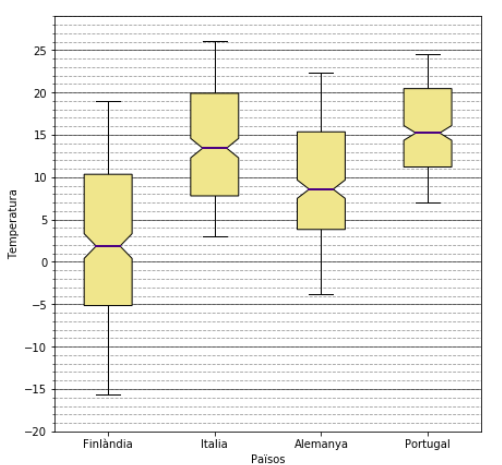
\includegraphics[width=0.5\textwidth]{../img/tempMitjaVariacioPaisos}
	\caption{Temperatures }
	\label{fig-tempMitjaPaisos}
\end{figure}

A més d'analitzar el \textit{DataSet} també ha estat necessari passar els països a dades numèriques, ja que Scikit-Learn no permet \textit{Strings} per entrenar els seus algorismes [14]. Aquesta acció s'havia de fer d'una manera que no convertís les variables en categòriques, és a dir, que l'algorisme no entengués que ser d'un país o d'un altre tenia una relació numèrica. Per fer-ho s'ha utilitzat un mètode de la mateixa llibreria de SciKit-Learn que transforma els \textit{String} en variables binàries, per tant si és d'un país, serà un 1 i si no ho és, serà 0.

Un cop sabent que el \textit{DataSet} era adequat per fer aquestes anàlisis, s'ha començat a escollir i entrenar diversos algorismes de regressió. Els algorismes de regressió són tasques d'aprenentatge inductiu [2]. Es diferencien en les tasques de classificació a causa del fet que en la regressió es prediuen valors numèrics, en canvi en la classificació es prediuen etiquetes de classe. La tasca de regressió consisteix en l'assignació de variables sobre un domini donat, aquestes variables estan descrites per atributs discrets. A partir d'aquest conjunt de dades, els algorismes de regressió assignen valors numèrics a instàncies d'aquest domini amb la finalitat d'aconseguir una aproximació a partir de valors que es donen~[15]. Dins de la regressió s'ha decidit agafar un conjunt de mètodes que es considerin dins de l'estat de l'art actual en temes de \textit{Machine Learning}.

\subsubsection{Arbres de Decisió:} Els arbres de decisió són models predictius no linears que serveixen per fer tasques de regressió i tasques de classificació. La idea és simple, si es vol predir una classe o resposta Y a partir d'entrades X cal fer créixer un arbre binari. En els nodes d'aquest arbre binari s'aplica un test sobre l'input que es consideri més rellevant, per exemple en la figura 2 es comença preguntant sobre la contaminació de CO$_2$. En aquest test es fa una pregunta binària de si o no, si la resposta és si es passarà al fill de la dreta, si la resposta és no, es passarà al fill de l'esquerra. A partir d'aquí, es van fent tests en cada un dels nodes, l'input que s'agafa per formular la pregunta pot variar segons les dades que s'estiguin treballant. Com es mostra a la figura 2 si s'envà cap a l'esquerra, es passa a testejar l'input de les emissions de CH$_4$. A la figura també es pot observar com les prediccions sobre quina és la temperatura final s'acaben fent en arribar a les fulles de l'arbre. Aquestes prediccions vénen donades pel conjunt de totes les preguntes que s'han anat formulant en els seus antecessors [16].
\begin{figure}[!h]
\centering
	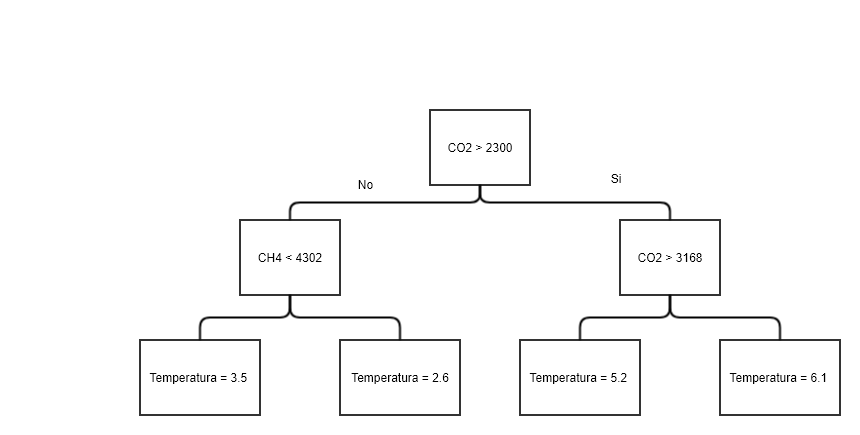
\includegraphics[width=0.5\textwidth]{../img/arbreDecisioSimple}
	\caption{Arbre de Decisió Bàsic}
	\label{fig-DecisionTree}
\end{figure}

Quan hi ha molts inputs a l'hora d'entrenar l'arbre de decisió, el mateix arbre ha d'escollir quin paràmetre dels inputs cal avaluar primer. Una mala elecció d'aquest input pot comportar que es comenci a fer comprovacions innecessàries, causant un impacte negatiu en l'eficiència de l'entrenament. L'arbre de decisió fa aquesta elecció a partir d'una recerca mitjançant la força bruta, en aquesta s'intenta buscar quina és la pregunta que pot aportar més informació de cara als següents nodes. Aquesta decisió la fa en cada un dels nodes i va variant fins a arribar a una fulla. Si en aquesta recerca es trobessin dues preguntes sobre dos inputs, que donen la mateixa quantitat d'informació, l'arbre escull una arbitràriament [16].

Per acabar, els arbres de decisions tenen molts paràmetres editables com la seva longitud màxima, el nombre màxim de fulles, el mínim nombre de paràmetres per considerar el node com una fulla... La majoria d'aquests paràmetres limiten el creixement de l'arbre, ja que per defecte creix fins a fer totes les preguntes possibles. Aquests paràmetres són molt importants en l'obtenció de bons resultats, parar el creixement d'un arbre, en una profunditat equivocada, pot fer que l'arbre acabi descartant gran part d'informació, ja que no tots els nodes donen la mateixa quantitat d'informació a l'arbre [16].
\subsubsection{Support Vector Machines:}
Support Vector Machines o SVM és un mètode d'aprenentatge supervisat que es pot utilitzar per a la classificació i la regressió. Aquest mètode té com a objectiu principal definir una funció f(x) que tingui com a molt una desviació o error per sota d'un límit establert en la creació del mètode. Per exemple, si s'estableix un error igual a 1, es descartaran tots els objectius amb un error superior a 1, i es consideraran tots els que tinguin un valor inferior. Un altre dels seus principals objectius consisteix en trobar un hiperpla de X dimensions, on X es el nombre de variables, que pugui separar òptimament els punts de les diferents classes. Un hiperpla òptim es considera quan aquest es troba a una distància màxima dels punts d'ambdues classes, els punts més proxims a aquests hiperplans s'anomenen \textit{Support Vectors}. Aquests punts són la clau en determinar la posició i orientació d'un hiperpla i determinar la distància màxima entre classes [17].

El SVM treballa amb productes sobre punts dins de dimensions definides, així troba les familiaritats entre dos vectors. Els SVM tenen un paràmetre essencial anomenat kernel, bàsicament són un conjunt de fórmules matemàtiques que defineixen com es processarà les dades que entren com a inputs. Els kernels són els encarregats de modificar el producte de punts establert pel SVM i adaptar-lo al seu espai. Per defecte el SVM té com a kernel el lineal, que limita el producte de punts original en dues dimensions. Si en lloc del lineal s'utilitzes un kernel com el polinòmic, aquest espai acceptaria també combinacions polinòmiques fins a certs graus, aconseguint fer paràboles [17]. 

A més d'aquests dos, hi ha un de molt utilitzat anomenat Radial Basis Function o RBF. Aquest utilitza un espai limitat per distribucions Gaussianes, en la majoria d'ocasions aquest kernel és el que pot arribar a obtenir els millors resultats [17]. Això es degut a que les funcions Gaussianes són més flexibles a l'hora de reballar amb diferents dimensions d'hiperplà. Per exemple, en la figura 3 es pot veure una petita prova per demostrar el comportament dels tres kernels més utilitzats. Aquí es pot veure clarament com els kernels lineas i polinomial no s'adequen bé amb un conjunt de dades que varia molt, en canvi el kernel RBF s'ha pogut adaptar millor a aquesta variació i ha pogut traçar una corba amb un error bastant baix. 
\begin{figure}[!h]
\centering
	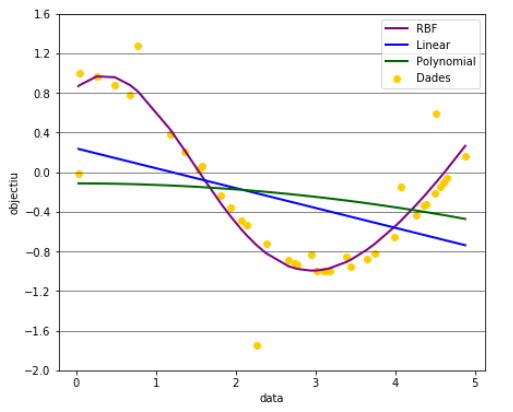
\includegraphics[width=0.5\textwidth]{../img/KernelsSVM}
	\caption{Comparació de kernels SVM}
	\label{fig-KernelsSVM}
\end{figure}

Cada un dels kernels té els seus paràmetres que modifiquen el seu comportament, per exemple, el kernel polinòmic té un anomenat \textit{degree} que modifica el grau del polinomi que s'utilitzarà per trobar el millor hiperplà. En el cas del RBF hi ha dos paramatres que determinen el seu percentatge d'encerts, aquests son C i \textit{gamma}.  
 \begin{itemize}
\item \textbf{C:} Com s'ha dit abans, les SVM pretenen aconseguir un marge màxim i tenir un error mínim de classificació. Aquest paràmetre es l'encarregat de determinar a que se li dona prioritat. Una C elevada seria correcte si es tinguès una funció de regressió que fes bones prediccions amb la majoria de punts amb els que s'entrena, per tant cal reduir el marge màxim ja que l'error es petit. En canvi una C petita convè si es té una funció de regressió més simple i que produeix més errors, llavors es necessita augmenta el marge màxim per incloure més punts.
\item \textbf{Gamma:} El comportament de SVM es molt sensible a aquest parametre ja que indica el radi d'influencia que tenen els \textit{Support Vector} a la resta del conjunt de dades. Per una banda, si aquest parametre es molt petit, l'algorisme no podrà entendre la complexitat total del conjunt de dades i es comportaria d'una forma semblant a un kernel linear, ja què aquest parametre li indicarà que pot agrupar la majoria d'ells amb el valor dels punts \textit{Support Vector}. Per l'altra, si es molt gran, es produiria una situació d'overfitting. El rang quedaria limitat al propi \textit{Support Vector} i no podria agrupar cap dels punts amb ell, per tant també produiria un error molt elevat.
\end{itemize}
\subsubsection{Random Forest:}
El Random Forest és un dels mètodes de ML que s'està utilitzant més en l'actualitat, com els altres dos, es pot utilitzar tant per classificació com per regressió. La idea principal del Random Forest és la de combinar diversos arbres de decisió iguals relacionats entre ells. Es basa en la idea de que la combinació de molts algoritmes iguals aconsegueix millors resultats que un de sol molt potent. Com es pot veure a la figura 4, que representa un Random Forest amb dos arbres, el mètode crea dos arbres de decisió i després combina els resultats de cada un d'ells mitjançant el \textit{Bagging Method} o un altre algoritme segons la implementació que s'esculli [19].Aquest mètode combina prediccions de múltiples algoritmes per aconseguir prediccions més exactes. El \textit{Bagging} es útil quan hi ha algoritmes amb una variancia molt elevada, com els arbres de decisió, i basicament aplica el mètode anomenat \textit{Bootstrap} a aquests algorismes.\textit{Bootstrap} s'encarrega d'agafar un nombre determinat de subconjunts de dades, dins del conjunt, i calcula la mediana del subconjunt. Un cop té totes les medianes agafa la mitjana de totes elles aconseguint el resultat final. 
\begin{figure}[!h]
\centering
	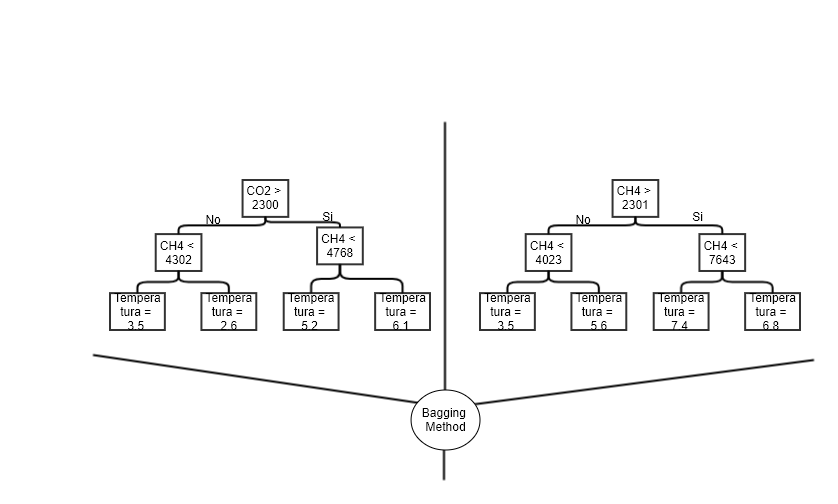
\includegraphics[width=0.5\textwidth]{../img/randomForest}
	\caption{Random Forest amb 2 arbres}
	\label{fig-RandomForest}
\end{figure}

El Random Forest té pràcticament els mateixos paràmetres que un arbre de decisió però amb petites diferències que optimitzen cada una de les decisions preses per l'arbre. Com s'ha dit anteriorment els arbres necessiten escollir quina pregunta s'ha de fer en cada node per aconseguir informació a l'hora de separar les variables. Aquesta situació fa que si s'agrupessin molts arbres junts tots acabarien sent practicament iguals, ja que tots escollirien la mateixa manera de separar. Aquest fet no aportaria una millora molt gran ja que al final el resultat seria pràcticament el mateix per tots els arbres i a l'hora d'agrupar-los la mitjana acabaria resultant aquell nombre. Per evitar això el Random Forest separa els inputs en subconjunts i cada arbre ha d'escollir de forma aleatoria el millor input per separar les dades. Així cada arbre acabarà tenint un subconjunt diferent d'inputs i els resultats seràn més dispersos, que permetrà adaptar-se més a qualsevol conjunt de dades a l'hora de predir [20].

El Random Forest permet editar molts paràmetres entre els quals destaquen:
 \begin{itemize}
\item \textbf{N\_estimators:} Permet modificar el número d'arbres de decisió abans de començar a aplicar el \textit{Bagging Method}.
\item \textbf{Min\_sample\_leaf:} Es igual al dels arbres de decisió i serveix per determinar el mínim número de mostres que es necessita per ser una fulla.
\item \textbf{Max\_depth:} Determina la profunditat màxima dels arbres de decisió.
\item \textbf{Min\_samples\_split:} Es igual al dels arbres de decisió i serveix per determinar el mínim número de mostres que es necessita per dividir un node.
\end{itemize}

\subsubsection{Xarxes Neuronals}
Actualment les xarxes neuronals són dels algorismes més prometedors en l'àmbit del \textit{Machine Learning} o \textit{Deep Learning}. Sobretot destaquen per la seva versatilitat, escalabilitat i una gran potència de còmput. Les més utilitzades, i que han demostrat millors resultats, han sigut les \textit{Multi Layer Perceptron} o MLP. Aquest tipus de xarxes es basen en la combinació de \textit{Perceptrons}, una de les arquitectures de xarxes neuronals més simples formada per una capa de \textit{Threshold Logic Unit} o TLU. Al cap i a la fi una MLP està formada per diverses capes de TLU amb una capa destinada a rebre les dades d'entrada, un conjunt de capes internes i una capa destinada a treure les prediccions [21]. Tal i com es pot veure a la figura 5 totes les neurones que formen part de la xarxa estan completament interconnectades entre elles, excepte l'última capa que només retorna els resultats. Aquí es pot veure com les capes poden tenir un número de neurones diferent, tot i això es recomana acabar amb una sola neurona si al final s'ha de retornar una unica predicció. També es pot observar els diferents tipus de capes dins d'una xarxa neuronal simple.
 \begin{figure}[!h]
\centering
	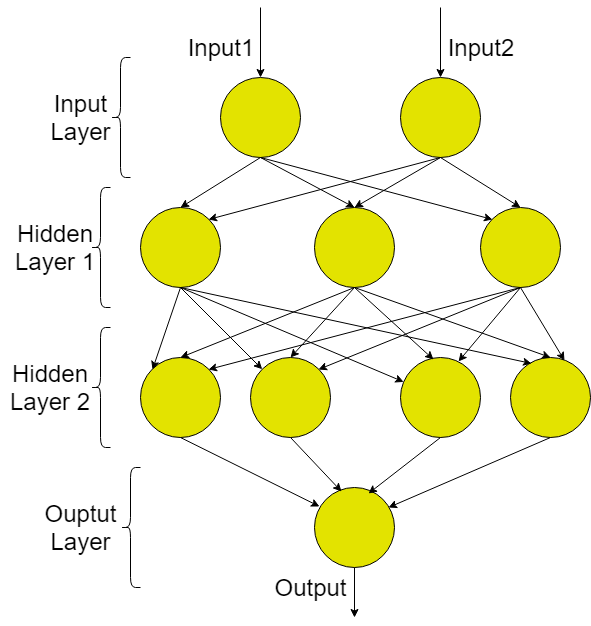
\includegraphics[width=0.5\textwidth]{../img/XarxaNeur}
	\caption{Xarxa Neuronal de 4 capes}
	\label{fig-XarxaNeur}
\end{figure}

Al començament es va decidir utilitzar les xarxes que ofereix la llibreria Scikit-Learn, de on s'han tret tots els algorismes anteriors, pero en aquest hi havia fortes limitacions que no permetien crear una xarxa decent que pogués demostrar totes aquestes característiques que la fan destacar. El principal inconvenient va sorgir quan a l'hora d'implementar la xarxa la llibreria no deixa editar cada capa individualment sinó tot el conjunt a la vegada, això limita molt el seu desenvolupament ja que moltes xarxes necessiten capes de diferent tipus, amb diferents neurones per poder exprimir al màxim el seu potencial. 

Degut a aquests inconvenients es va decidir buscar una alternativa millor, i aquesta ha acabat sent la API de Keras. Keras treballa sobre TensorFlow, un framework dedicat especialment pel Machine Learning que es troba en l'estat de l'art d'aquest àmbit, però nomès fica una capa per sobre d'ell per tal de facilitar l'implementació d'algorismes mantenint totes les avantatges del framework. Amb aquesta API si que s'ha pogut probar diferents models de xarxes amb capes de diferents neurones i amb diferents funcions d'activació. 

Una xarxa neuronal és molt més extensa d'editar que els altres algorismes, degut a la seva gran quantitat d'hiperparametres i la diversitat entre les combinacions entre ells. Per començar s'ha hagut de limitar la recerca a xarxes simples, degut a que no es podia dedicar masses hores a un sol algorisme. En aquest cas nomès s'han contemplat els models sequencials de Keras, que funcionen sense problemes per tots els casos i amb bons resultats. També s'ha hagut de tenir una limitació en el número de capes per tal de no complicar massa la xarxa, en aquest cas no s'ha volgut superar les 5 capes, més que suficient per la quantitat de dades que conté el \textit{DataSet}. A partir d'aquí tota la resta d'hiperparametres s'ha deixat sense limitacions.

Entre els paràmetres hi ha uns quants que cal destacar per l'afectació que té en el comportament d'una xarxa:
 \begin{itemize}
\item \textbf{Activation:} Aquest parametre es el més rellevant de tots ja que decideix quan es considera una neurona activada, i quan no. Per exemple es pot ficar un límit i si una neurona el supera es considera activada, si no es considera desactivada, aquest seria l'activació binaria o \textit{Step Function}. També hi ha la linear on l'activació es proporcional als inputs o neurones del sistema. Una altra bastant utilitzada es la Relu que té un comportament semblant a al linear pero considerant com a funció d'activació qualsevol valor positiu superior a 0 [21].
\item \textbf{Batch\_size:} Es el nombre de mostres que es propagaran al llarg de la xarxa. Per exemple, si es té un conjunt de 1000 dades, pero aquest parametre es 100, s'aniran agafant subconjunts de 100 i s'aniran propagant per la xarxa. Com més petit sigui el valor més inexacte serà la xarxa.
\item \textbf{Ephochs:} Són el número de cops que es propagaran totes les dades per la xarxa. Si es té un batch\_size molt petit i un epoch molt gran es necessitarna moltes iteracions per acabar d'entrenar-la.
\end{itemize}

\subsubsection{SearchCV}
D'aquests algorismes s'ha fet un entrenament amb els paràmetres per defecte marcats per la llibreria de Scikit-Learn i després s'ha utilitzat dues tècniques, molt utilitzades en l'àmbit del ML per trobar el conjunt de paràmetres més òptim per cada algorisme. Aquestes tècniques tenen com a objectiu esprémer al màxim els algorismes i aconseguir l'aproximació més precisa de la temperatura. Aquestes tècniques han estat:
 \begin{itemize}
\item \textbf{Grid SearchCV:} Implementa una recerca exhaustiva dels paràmetres editables d'un mètode de predicció. Un cop fet aquest anàlisis entrena l'algorisme amb la millor combinació de paràmetres que ha trobat. Amb cada una de les combinacions fa 3 iteracions i després utilitza una fórmula per avaluar el resultat obtingut, aquest pot ser el Mean Absolute Error o MAE, Mean Squared Error [22]... Les iteracions dels paràmetres les fa en ordre ascendent, comença pels paràmetres més petits i va augmentant-los fins al límit que se l'hi ha establert.
\item \textbf{Randomized SearchCV:} És un mètode molt semblant al Grid Search. També fa una recerca sobre els millors paràmetres que aconsegueixin treure el millor resultat del mètode. La principal diferència és que en lloc de fer-ho de forma iterativa i ascendent ho fa de forma iterativa però aleatòriament. Això permet que es puguin provar valors molt elevats sense necessitat de què la recerca augmenti exponencialment el temps necessari per acabar [23].
\end{itemize}
\section{Resultats}
Per aconseguir els millors resultats amb cada un dels algorismes s'han fet proves exhaustives amb el Randomized Search. En el cas de les Xarxes Neuronals no s'ha pogut utilitzar el mateix metode degut a que 
Per aconseguir els resultats s'ha hagut d'aplicar tant el Grid Search com el Randomized Search amb les mateixes iteracions als quatre algorismes escollits, amb els mateixos conjunts de dades per cada un d'ells. En tots els casos els millors resultats els ha donat la tècnica de Randomized Search. Això s'ha donat a causa del fet que la tècnica pot arribar a paràmetres molt més grans i diversos. El Grid Search no pot fer el mateix pel fet que el Randomized utilitza iteracions de valors aleatoris, dins d'un rang molt més gran de valors. En canvi, el Grid Search està limitat a anar fent proves seqüencialment, començant pels valors més petits i fins a arribar al màxim del rang que s'ha establert. Al cap i a la fi el Grid Search està limitat per la quantitat elevada de càlculs que necessita fer. Per exemple, ficant el mateix nombre de variables, amb el mateix rang de valors en cada una d'elles, per arribar al valor màxim el Grid Search ha de fer X iteracions prèvies (on X pot ser un número molt elevat d'iteracions), en canvi el Randomized ho pot fer a la primera sense passar per totes les anteriors.

A la taula número 3 es pot veure una comparativa amb els 4 algorismes anal·litzats, la millor combinació d'hiperparàmetres per cadascun d'ells i el Mean Absolut Error de cada una de les combinacions. EXPLICAR TAULA I PERQUE MAE.

Com es pot veure a la figura 4 l'algorisme que ha aconseguit aproximar-se més als valors originals ha estat el Random Forest, en canvi el pitjor ha estat l'algorisme de les Support Vector Machine.
\begin{figure}[!h]
\centering
	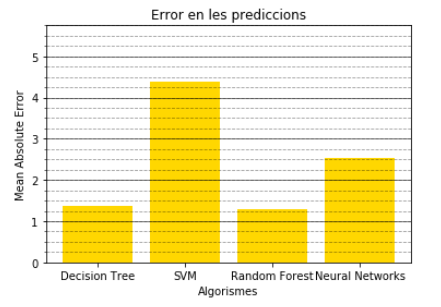
\includegraphics[width=0.5\textwidth]{../img/comparacioMetricsAlgs}
	\caption{MAE dels mètodes}
	\label{fig-Metrics}
\end{figure}
 EXPLICAR COMPORTAMENT SVM I XARXES I COMPARATIVA DEL COMPORTAMENT DE TOTS (LES XARXES FALLEN MOLT EN ALGUNE SI ALTRES DIUEN EXACTAMENT EL MATEIX)

Aquests resultats són molt bons a causa del fet que l'error és bastant baix, considerant que la temperatura varia d'un any per l'altre entre 2 i 4 graus. No obstant això, els dos mètodes tenen un comportament una mica diferent a l'hora de fer prediccions. El Random Forest manté bastant la constància amb les temperatures que no varien massa, en canvi sí que falla bastant quan hi ha un canvi brusc de temperatura. Per l'altra banda els Decision Tree fallen en la gran majoria de prediccions però amb un error baix en tots ells, això fa que el MAE d'ambdós sigui molt semblant, encara que el Random Forest acabi tenint un més baix.
\begin{figure}[!h]
\centering
	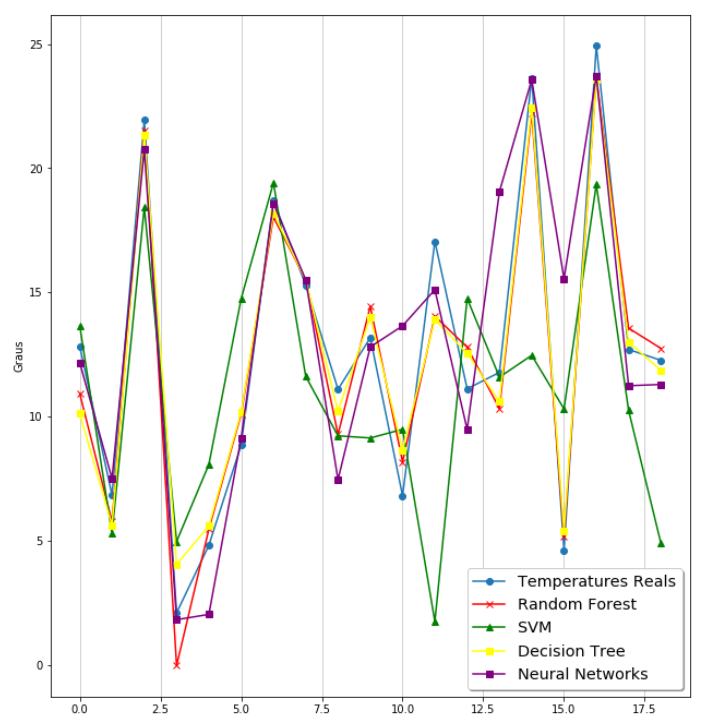
\includegraphics[width=0.5\textwidth]{../img/comparacioAlgs}
	\caption{Comportament dels mètodes}
	\label{fig-temps}
\end{figure}

\section {Conclusions}
En aquest treball s'ha pogut complir tots els objectius proposats, excepte el de trobar la millor configuració de cada un d'ells. 
\section{Treball Futur}
Com a idees per continuar aquest TFG es podria fer la mateixa anàlisi de les dades però en un àmbit mundial en lloc d'Europeu. Segurament els resultats siguin encara millors gràcies a un nombre més gran de dades a analitzar. Degut a que s'han vist diversos algorismes i s'ha hagut de fer el propi \textit{Dataset}, no ha sigut possible treballar amb molt de detall algorismes dins de l'estat de l'art del ML,com les SVM i les Xarxes Neuronals. Una línia de treball molt interessant pot ser fer un anàlisis exhaustiu amb algun d'aquests algorismes en un \textit{Dataset} ja preparat. Si es pot exhaustivament poden sortir resultats molt interessants amb alguns \textit{Datasets} del canvi climàtic, o tambè d'un altre àmbit.

Més enllà dels mètodes de Big Data, Machine Learning o aconseguir bons algorismes de regressió, aquest treball també pot acabar sent una bona base perquè apareguin més treballs relacionats amb el canvi climatic ja què aquest tema es pot aprofitar per aconseguir treballs molt prometedors com, per exemple, montar uns sensors que detectin quin nivell de contaminació hi ha en un lloc determinat, una aplicació que t'indiqui on va cada residu i fomentar el reciclatge...
\begin{thebibliography}{11}
\bibitem{1}
\url{https://earthobservatory.nasa.gov/world-of-change/DecadalTemp}
\bibitem{2}
"Sample Research", \textit{The Standish Group}.~[En~línia].~Disponible~a:~\url{https://www.standishgroup.com/sample_research}~[Accedit~Octubre~4,~2018].
\bibitem{3}
"Scrum Reference Card now available in English and Spanish",  \textit{Agile Methodology}. [En línia]. Disponible a: \url{http://agilemethodology.org/ }. [Accedit Octubre 4, 2018].
\bibitem{4}
"The Complete Guide to Understanding Agile Testing", \textit{QA Symphony}. [En línia].Disponible a: \url{https://www.qasymphony.com/blog/agile-methodology-guide-agile-testing/}. [Accedit Octubre 4, 2018].
\bibitem{5}
``Climate Change: Earth Surface Temperature Data”, \textit{Berkeley Earth}. [En línia]. Disponible a: \url{ https://www.kaggle.com/unitednations/international-greenhouse-gas-emissions}. [Accedit Novembre 9, 2018].
\bibitem{6}
 ``International Greenhouse Gas Emissions”, \textit{United Nations}. [En línia]. Disponible a: \url{ https://www.kaggle.com/unitednations/international-greenhouse-gas-emissions}. [Accedit Novembre 9, 2018].
\bibitem{7}
 ``Land Use, Land-Use Change and Forestry (LULUCF)", \textit{United Nations}. [En línia]. Disponible a: \url{ https://unfccc.int/topics/land-use/workstreams/land-use--land-use-change-lulucf}. [Accedit Novembre 7, 2018].
\bibitem{8}
Federica Pozzi, ``Importancia del recuento del UTCUTS (LULUCF) para el éxito del Acuerdo de París". \textit{Carbon Market Watch}. [En línia]. Disponible a: \url{https://carbonmarketwatch.org/es/2017/07/18/29671/}. [Accedit Novembre 7, 2018].
\bibitem{9}
``Databricks Unified Analytics", \textit{DataBricks}. [En línia]. Disponible a: \url{https://databricks.com/}. [Accedit Novembre 6, 2018].
\bibitem{10}
 ``Python Data Analysis Library", \textit{Pandas}. [En línia]. Disponible a: \url{https://pandas.pydata.org/}. [Accedit Novembre 7, 2018].
\bibitem{11}
F.Julbe, \textit{Anàlisi de dades massives: Tècniques fonamentals}. Barcelona, UOC. Pàgines: 30-32.
\bibitem{12}
B.Fornberg, J.Zuev. \textit{The Runge phenomenon and spatially variable shape parameters in RBF interpolation}. University Of Colorado.
\bibitem{13}
 ``Interpolation", \textit{Wikipedia}. [En línia]. Disponible a: \url{https://en.wikipedia.org/wiki/Interpolation#Spline_interpolation}. [Accedit Novembre 10, 2018].
\bibitem{14}
``Encoding Categorical Features", \textit{Scikit-Learn}. [En línia]. Disponible a:\url{https://scikit-learn.org/stable/modules/preprocessing.html#encoding-categorical-features}. [Accedit Desembre 22, 2018].
\bibitem{15}
F.Julbe, \textit{Anàlisi de dades massives: Tècniques fonamentals}. Barcelona, UOC. Pàgines: 43-45.
\bibitem{16}
R. Tibshirani, \textit{Classication and Regression Trees}. Machine Learning Department, Carnegie Mellon University. 2009.
\bibitem{17}
Alex J. Smola, B. Schölkopf, \textit{A tutorial on support vector regression}. RSISE, Australian National University. 2003.
\bibitem{18}
\url{https://scikit-learn.org/stable/auto_examples/svm/plot_rbf_parameters.html}
\bibitem{19}
``Kernel Functions-Introduction to SVM Kernel \& Examples", \textit{Data Flair}. [En línia]. Disponible a:\url{https://towardsdatascience.com/the-random-forest-algorithm-d457d499ffcd}. [Accedit Desembre 22, 2018].
\bibitem{20}
L. Breiman, \textit{Random Forests}. Statistics Department, University of California Berkeley. 2001.
\bibitem{21}
A.Géron, \textit{Hands-On Machine Learning with Scikit-Learn \& TensorFlow}. Sebastopol, CA: O’Reilly Media, 2017. Capitol 10.
\bibitem{22}
``Grid Search CV", \textit{Scikit-Learn}. [En línia]. Disponible a:\url{https://scikit-learn.org/0.15/modules/generated/sklearn.grid_search.Grid SearchCV.html#sklearn.grid_search.Grid SearchCV}. [Accedit Desembre 22, 2018].
\bibitem{23}
``Randomized Search CV", \textit{Scikit-Learn}. [En línia]. Disponible a:\url{https://scikit-learn.org/stable/modules/generated/sklearn.model_selection.Randomized SearchCV.html}. [Accedit Desembre 22, 2018].

\end{thebibliography}
\clearpage
\section{Annex}
 \begin{itemize}
\item \textbf{Temperatures Italia:}
\begin{figure}[!h]
\centering
	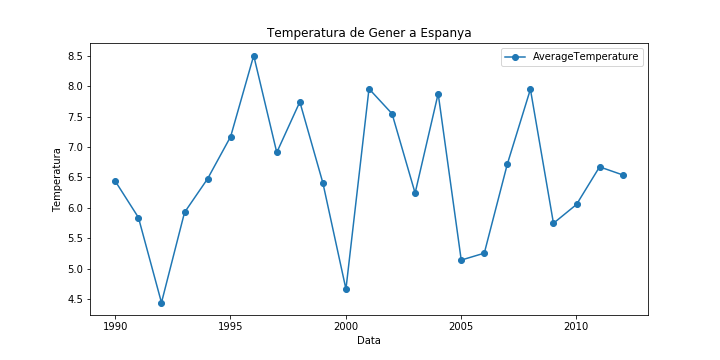
\includegraphics[width=1\textwidth]{../img/tempSpain}
	\caption{Temperatura a Espanya}
	\label{fig-tempSpain}
\end{figure}
\item \textbf{Temperatures Alemanya:}
\begin{figure}[!h]
\centering
	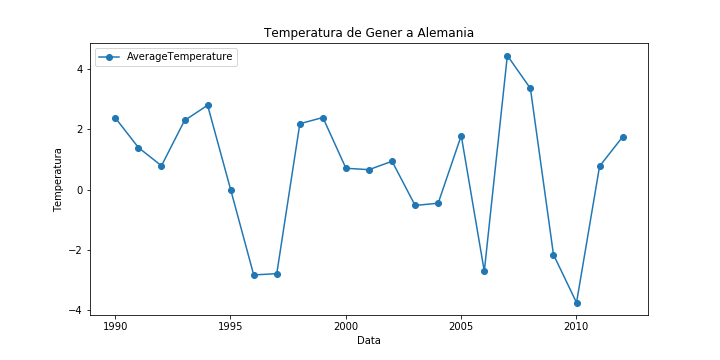
\includegraphics[width=1\textwidth]{../img/tempGermany}
	\caption{Temperatura a Alemanya}
	\label{fig-tempGerm}
\end{figure}
\end{itemize}
\end{document}

